%
% report.tex - tex model of graduation work
% Version 0.1
%
% Author: Paulo S. Machado
% Date: 2S 2011
%
% Release under de GNU Public License v3.0 or greater
% This library is free software; you can redistribute it and/or
% modify it under the terms of the GNU General Public
% License as published by the Free Software Foundation; either
% version 3.0 of the License, or (at your option) any later version.
% 
% This template is distributed in the hope that it will be useful,
% but WITHOUT ANY WARRANTY; without even the implied warranty of
% MERCHANTABILITY or FITNESS FOR A PARTICULAR PURPOSE.  See the GNU
% General Public License for more details.
% 
% You should have received a copy of the GNU Lesser General Public
% License along with this template; if not, write to the Free Software
% Foundation, Inc., 51 Franklin St, Fifth Floor, Boston, MA  02110-1301  USA
%
\documentclass[a4paper,11pt]{article}

%
% preamble.tex - tex model of graduation work
% Version 0.1
%
% Author: Paulo S. Machado
% Date: June 2010
%
% Release under de GNU Public License v3.0 or greater
% This library is free software; you can redistribute it and/or
% modify it under the terms of the GNU General Public
% License as published by the Free Software Foundation; either
% version 3.0 of the License, or (at your option) any later version.
% 
% This template is distributed in the hope that it will be useful,
% but WITHOUT ANY WARRANTY; without even the implied warranty of
% MERCHANTABILITY or FITNESS FOR A PARTICULAR PURPOSE.  See the GNU
% General Public License for more details.
% 
% You should have received a copy of the GNU Lesser General Public
% License along with this template; if not, write to the Free Software
% Foundation, Inc., 51 Franklin St, Fifth Floor, Boston, MA  02110-1301  USA
%
% Language
\usepackage[portuges,brazil]{babel}
\usepackage[top=3cm,bottom=3cm,left=3.0cm,right=3cm]{geometry}
\usepackage[pdftex]{graphicx}
\usepackage{listings}
\usepackage{textcomp}
\usepackage{amssymb}
\usepackage{amsmath}
\usepackage{color}
% Encoding
\usepackage[utf8]{inputenc}

%\usepackage{wrapfig}
%\usepackage{hyperref}

% This will commands into the pdf to create a linked table of contents, as well
%as links for 
% the cross-references such as calls to figure and page numbers 
\usepackage[pagebackref=true]{hyperref}  
\hypersetup{
  pdftitle     = Trabalho de Graduação,
  pdfauthor    = Paulo Silveira Machado,
  colorlinks   = true,
  linkcolor    = black,
  anchorcolor  = red,
  citecolor    = blue,
  filecolor    = red,  
  urlcolor     = red
}



\DeclareGraphicsExtensions{.jpg,.jpeg,.png}
\graphicspath{{../../imagens/}}
% Heading foot
\usepackage{fancyhdr}
\pagestyle{fancy}
\headheight 15pt
\renewcommand{\sectionmark}[1]{\markright{\thesection\ #1}}
\rhead[\fancyplain{}{\bfseries\thepage}] %
    {\fancyplain{}{\bfseries\rightmark}}
\lhead{}
%\lhead[\fancyplain{}{\scshape\leftmark}] %
%    {\fancyplain{}{\bfseries\thepage}}
\cfoot{--~\thepage~--}


\begin{document}

% Title page and table of contents
%
% title.tex - tex model of graduation work
% Version 0.1
%
% Author: Paulo S. Machado
% Date: June 2010
%
% Release under de GNU Public License v3.0 or greater
% This library is free software; you can redistribute it and/or
% modify it under the terms of the GNU General Public
% License as published by the Free Software Foundation; either
% version 3.0 of the License, or (at your option) any later version.
% 
% This template is distributed in the hope that it will be useful,
% but WITHOUT ANY WARRANTY; without even the implied warranty of
% MERCHANTABILITY or FITNESS FOR A PARTICULAR PURPOSE.  See the GNU
% General Public License for more details.
% 
% You should have received a copy of the GNU Lesser General Public
% License along with this template; if not, write to the Free Software
% Foundation, Inc., 51 Franklin St, Fifth Floor, Boston, MA  02110-1301  USA
%
% Title page
\begin{titlepage}
\begin{center}
 
% Header

\includegraphics[width=0.15\textwidth]{figures/unicamp128}\\[1cm]
\textsc{\LARGE Universidade Estadual de Campinas}\\[0.3cm]
\textsc{\LARGE ES952 - Trabalho de Graduação II}\\[3.0cm] 
\textsc{\Large Relatório de Atividades} \\[0.2cm]

  
% Title
\hfill
\textsf{ \LARGE \bfseries Desenvolvimento de um câmbio automático para
bicicletas}

\vfill
% Author and project
\begin{minipage}{0.49\textwidth}
\begin{flushleft} \large
\emph{Autor:}\\
Paulo Silveira Machado \\
RA: 024831
\end{flushleft}
\end{minipage}
\begin{minipage}{0.5\textwidth}
\begin{flushright} \large
\emph{Orientador:} \\
Prof. Dr. Luiz Otávio Saraiva Ferreira\\
Faculdade de Engenharia Mecânica
\end{flushright}
\end{minipage}
 
\vfill
 
% Botton
{\large 2\textordmasculine ~Semestre/2011}
\end{center}
 
\end{titlepage}

% Table of contents
\tableofcontents
\pagebreak

% List of figures
\listoffigures
\pagebreak

% List of tables
\listoftables
\pagebreak

\lstset{frame=single,
    showstringspaces=false,
    extendedchars=true,
    language=C++,
    backgroundcolor=\color[rgb]{0.95,0.95,0.95},
    rulecolor=\color[rgb]{0.3,0.3,0.3},
    basicstyle=\scriptsize\ttfamily,
    commentstyle=\color[RGB]{105,105,105}\rmfamily\itshape,
    keywordstyle=\color[rgb]{0.6,0.0,0.0}\bfseries,
    stringstyle=\color[rgb]{0.6,0.4,0.4},
    identifierstyle=\color[rgb]{0.0,0.0,0.5},
    basicstyle=\tiny,
}

%%%
%
\section{Resumo}
\label{sec:resumo}
% Breve contexto, função
% Pré requisitos
% Estrutura do documento
% Do que se trata
% Estrutura do texto
A ideia deste projeto surgiu das observações diárias de ciclistas e do uso
da bicicleta, onde grande parte das pessoas não sabe utilizar de
forma eficiente as marchas de suas bicicletas. Estas parecem ser
complicadas (\textit{mountain bikes} simples possuem pelo menos 18 marchas) e de
difícil manejo e configuração. Assim como em uma transmissão automotiva, maus
hábitos no seu manejo -- esticar marchas, manter a mão apoiada sobre a alavanca,
entre outros -- causam desgaste precoce dos componentes, esforços desnecessários
(neste caso para ciclista) e até risco de segurança.
\\
O benefício primordial de qualquer automação (i.e. retirar do usuário o
controle ou parte do controle sobre o sistema que interage) é a melhora no
fluxo do processo devido ao grande controle que tem se sobre o sistema. Os
resultados deste benefício são, em alto nível, o aumento da qualidade,
repetibilidade e uniformidade, aplicação de estratégias ótimas de controle e
simplicidade na interação com utilizador.
\\
Este relatório apresenta o desenvolvimento e resultados do trabalho proposto e
estudado na primeira disciplina de Trabalho de Graduação: a construção de um
protótipo funcional de um sistema de troca de marchas automatizados para
bicicletas convencionais. Neste primeiro trabalho foram construídas as base
teóricas e ferramentais para a construção de um protótipo funcional: construção
da bancada experimental; desenvolvimento da lógica; e estudo de soluções 
existentes. Ou seja, dados os objetivos do projeto -- software de controle,
circuito de controle, atuados mecânico e a junção destes no protótipo --
apresenta-se o caminho percorrido até o objetivo e os resultados alcançados.
\\
O documento foi estruturado de forma a descrever o problema de engenharia, as
alternativas consideradas, escolhas e desenvolvimento de cada parte funcional do
protótipo final.


\pagebreak
%%%
%
\section{Introdução}
\label{sec:intro}
Automação ou Controle? Esta foi a tônica do início do projeto. A solução de
controle, mais elegante, mostrou-se pouco tangível devido a dificuldade de
modelar o sistema mecânico completo e logo foi abandonada.

\pagebreak
%%%
%
\section{Desenvolvimento das partes}
\label{sec:partes}
O projeto foi dividido em partes, com desenvolvimento em paralelo, para agilizar
o processo e para que mudanças no projeto de alguma das partes refletissem
imediatamente nas outras. Esta sinergia foi mais forte entre o Circuito de
controle (Sec. \ref{sec:arduino}) e o Software de controle (Sec.
\ref{sec:software}).

\subsection{Bancada experimental}
\label{sec:bancada}
Criar uma bancada para este projeto sempre foi uma das premissas básicas, tanto
que constituía um dos objetivos da primeira parte deste trabalho de graduação.
Simular os sinais do sistema via algum tipo de software ou kit não foi
considerada como opção, pois nenhuma nuance de um sistema real deveria ser
perdida. Logo a solução elaborada no primeiro trabalho foi usar uma bicicleta
convencional e transformá-la adequadamente. O resultado é apresentado na Figura
\ref{fig:bancada}.
\begin{figure}[ht]
 \begin{center}
  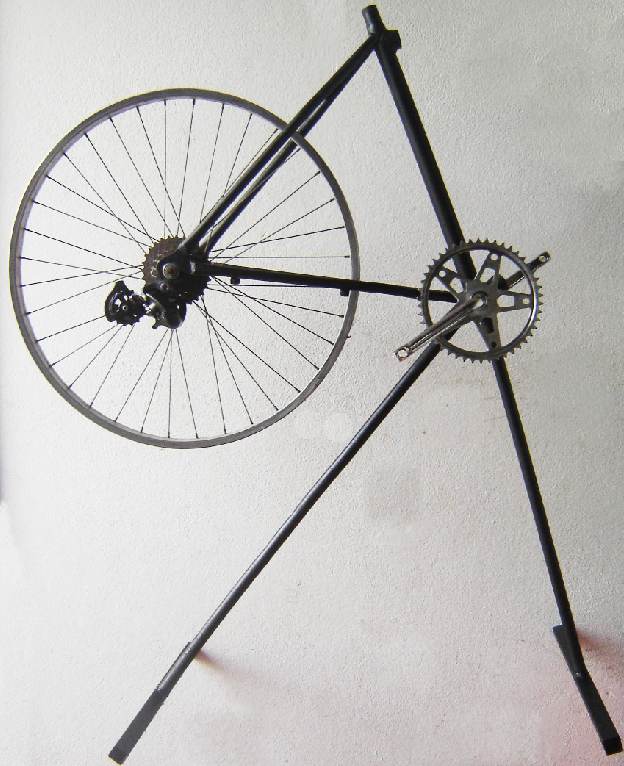
\includegraphics[width=4in]{bancada_tratada}
 \end{center}
 \caption{Bancada experimental - TG I}
 \label{fig:bancada}
\end{figure}
Ou seja, a bancada é uma meia bicicleta - com a parte traseira, onde estão os
elementos da transmissão  -- onde foram soldados apoios, possibilitando
``pedalar no vazio'' e realizar os testes do projeto, fiel a um cenário real. \\
Os problemas relativos a bancada foram muitos e surgiram no momento prévio aos
testes, quando os componentes da transmissão foram montados. As peças
disponíveis não foram escolhidas corretamente (corrente curta, coroa dianteira
não casou com o corrente), o que causou novos custos e atraso nos testes.

%%%
%
\subsection{Circuito de controle}
\label{sec:arduino}
Arduino\\
botões da constante K \\
Display LCD \\
debounce em hardware e software \\
comunicação serial \\
foto da montagem \\
circuito do pwm \\

%%%
%
\subsection{Software de controle}
\label{sec:software}
No início do projeto houve a intenção de usar técnicas de controle discreto no algoritmo de controle.
Porém a grande dificuldade de modelar o problema físico levou a uma mudança de
abordagem, do problema de controle para o problema de automação. Assim, baseado
nas entradas e saídas do sistema a lógica apresentada na Figura
\ref{fig:fluxograma1} foi elaborada, ainda na primeira parte deste trabalho.
% Fluxograma
\begin{figure}[ht]
 \begin{center}
  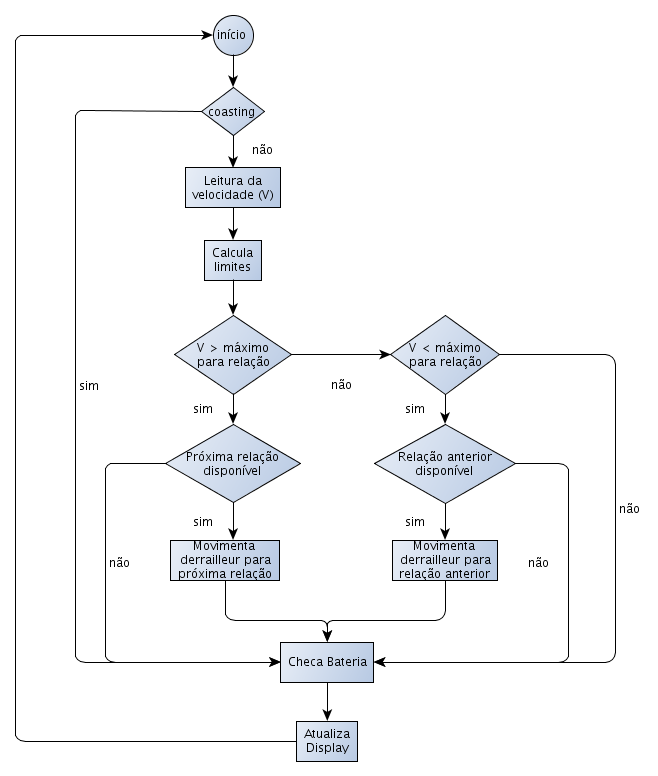
\includegraphics[width=4in]{fluxograma1}
 \end{center}
 \caption{Lógica de controle inicial}
 \label{fig:fluxograma1}
\end{figure}
Após o início da codificação, algumas 
% evolução da lógica
%TODO fluxograma da máquina de estado

%estrutura do código biblioteca e codigo
 
%%%
%
\subsection{Protótipo}
\label{sec:prototipo}


\pagebreak
%%%
%
\section{Testes e Resultados}
\label{sec:resultados}

\pagebreak
%%%
%
\section{Conclusões}
\label{sec:conclusoes}
% dificuldades
% trabalhos futuros (dinamo e gerenciamento de energia, memoria persistente, ajuste das relações)


\pagebreak
%%%
%
\section{Anexos}
\label{sec:anexos}

%%%
%
\subsection{Elementos sensores}
\label{sensores}
A definição e uso de elementos sensores foi um dos grandes obstáculos deste
projeto. Estes deveriam ser usados para a leitura de pulsos a cada revolução da
roda e do pedivela, gerando a informação de velocidade básica ao algoritmo de
controle. As soluções analisadas foram:
\begin{itemize}
 \item Sensor capacitivo
 \item Sensor indutivo
 \item \textit{Reed switch}
 \item Sensor de efeito HALL
\end{itemize}
Os principais critérios de escolha, que permearam o projeto desde sua concepção,
foram simplicidade e custo. Logo, foi feita a escolha pelo reed switch, o
mais simples e barato entre todos. \\
Porém, os \textit{reed switch} são chaves que geram muito ruído
(\textit{bounce}) o sinal gerado precisa de um tratamento para que possa ser
aproveitado. Foi considerado realizar o \textit{debounce} do sinal de duas
formas: via software; ou via hardware. A primeira foi logo descartada pois as
funções do programa responsáveis pelo cálculo de velocidade seriam rotinas de
interrupção, ou seja, eles devem ter uma execução muito breve, caso contrário
podem afetar a contagem de tempo do sistema. Uma função de \textit{debounce} em
software envolve, inerentemente algum \textit{delay}.\\

\begin{figure}[ht]
 \begin{center}
  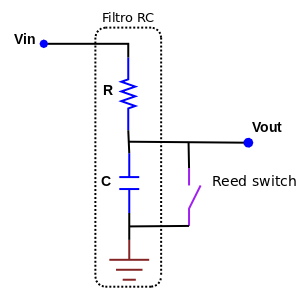
\includegraphics[width=1.8in]{lowpass}
 \end{center}
 \caption{Filtro passa-baixa passivo}
 \label{fig:lowpass}
\end{figure}

A única saída foi mesmo implementar o \textit{debounce} em hardware, utilizando
um filtro passa-baixa passivo, que usa apenas um resistor e um capacitor, de
acordo com o esquema da Figura \ref{fig:lowpass}. O ruído de um \textit{reed
switch} comum está na faixa de 1500Hz a 2000Hz\cite{reed}. É possível estimar a
frequência máxima ($f_{max}$) de ativação dos \textit{reeds} a partir de um
limite de velocidade da roda ($v_{max} = 90 km/h = 25 m/s$):
\begin{equation}
  v = \omega r = 2\pi f r \Rightarrow v_{max} = 2\pi f_{max} r
\end{equation}
O diâmetro da roda com pneu foi medido em d =65cm = 0.65m. Portanto, para velocidade máxima de 90 km/h:
\begin{equation}
  f_{max} = \frac{\displaystyle v_{max}}{\displaystyle \pi d} =
\frac{\displaystyle 25}{\displaystyle \pi 0.65} = 12.243 Hz
\end{equation}
Tomando a frequência de corte ($f_{c}$) dada pela relação,
\begin{equation}
  f_{c} = \frac{\displaystyle 1}{\displaystyle 2\pi\tau} \text{, onde } \tau =
RC
\end{equation}
igual a frequência máxima ($f_{max}$), diversas combinações de resistores e
capacitores são possíveis. Logo, o script \ref{code:lowpass} escrito em
pyhton\cite{python} foi usado para ajudar a dimensionar os componentes, de
acordo com o que foi adquirido (Sec. \ref{custos}) e o que foi
obtido.


%%%
%
\subsection{Elemento atuador}
\label{atuador}
Duas perguntas foram elaboradas para ajudar na definição de um atuador: Qual a
forma mais simples de atuar sobre um cabo utilizando um motor rotativo? Qual
tipo de motor é confiável e fácil de controlar? As repostas são,
respectivamente, uma polia e servo motor. \\
O raio da polia foi dimensionado de tal forma que, dado que um servo motor
rotaciona 180\textdegree, meia circunferência da polia seja deslocamento
suficiente para movimentar o derailleur da menor a maior marcha. Assim,
definimos o raio da polia ($r_{polia}$), o número de marchas (n) e o passo (p)
como o deslocamento necessário do cabo de comando para a mudança de uma marcha
consecutiva, de tal forma que:
\begin{equation*}
  \frac{\displaystyle 2\pi r_{polia} }{\displaystyle 2} = (n-1)p
\end{equation*}
\begin{equation}
  r_{polia} = \frac{\displaystyle (n-1)p}{\displaystyle \pi}s
\end{equation} 
Para a bancada de testes, n=6 e p=%TODO passo do cabo bancada.
\\O servo motor escolhido foi um Futaba S3004, tal qual o da Figura \ref{fig: servo}. Este possui rolamentos de esferas no eixo de saída, e torque de 4.1kg-cm a 6 volts. O servo drena muita corrente e gera bastante ruído, e portanto teve sua alimentação isolada.

\begin{figure}[ht]
 \begin{center}
  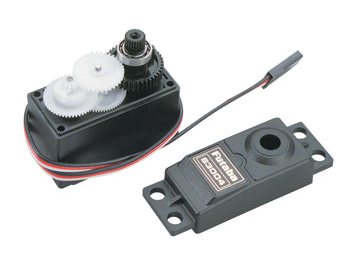
\includegraphics[width=3in]{S3004}
 \end{center}
 \caption{Servo Futaba S3004}
 \label{fig: servo}
\end{figure}



%%%
%
\subsection{Custos do Projeto}
\label{custos}
Os custos dos materiais utilizados foram relativamente baixos. O
reaproveitamento de componentes previamente adquiridos, e principalmente, o
baixo custo dos componentes envolvidos possibilitaram minimizar esta soma. A
Tabela \ref{tab:custos} a seguir computa os componentes e ferramentas.
{
\newcommand{\mc}[3]{\multicolumn{#1}{#2}{#3}}
\begin{table}[ht]
\begin{center}
\caption{Custos do projeto}
\label{tab:custos}
\begin{tabular}{lc}
\mc{1}{c}{\textbf{Material}} & \textbf{Preço (R\$)}\\\hline
Movimento central & R\$ 12,00\\
Arduino Duemilenove & R\$ 40,00\\
Servo Futaba s3004 & R\$ 12,00\\
Ferro de solda 100W & R\$ 18,00\\
\textit{Reed switch} (5x) & R\$ 3,45\\
Resistores 10k (6x) & R\$ 0,78\\\hline
\textbf{Total} & \textbf{R\$ 86,23}\\\hline
\end{tabular}
\end{center}
\end{table}
}



%%%
%
\subsection{Código Fonte}
\label{codigo}

\subsubsection{API da Biblioteca \textit{BikeTransmission}}
\label{code:api}
\textit{BikeTransmission.h}:
\lstinputlisting{../BikeTransmission/BikeTransmission.h}

\subsubsection{Implementação da Biblioteca \textit{BikeTransmission}}
\label{code:impl}
\textit{BikeTransmission.cpp}:
\lstinputlisting{../BikeTransmission/BikeTransmission.cpp}

\subsubsection{Programa principal}
\label{code:main}
\textit{principal.pde}
\lstinputlisting{../principal/principal.pde}

\subsubsection{\textit{Scripts} auxiliares}
\label{code:helper_scripts}

\lstset{frame=single,
    language=Python,
    basicstyle=\ttfamily\small,
    otherkeywords={=, +, [, ], (, ), \{, \}, :},
    keywordstyle=\color{blue},
    stringstyle=\color{red},
    showstringspaces=false,
    emph={class, pass, in, for, while, if, is, elif, else, not, and, or,
    def, print, exec, break, continue, return},
    emphstyle=\color{black}\bfseries,
    emph={[2]True, False, None, self},
    emphstyle=[2]\color{key},
    emph={[3]from, import, as},
    emphstyle=[3]\color{blue},
    upquote=true,
    morecomment=[s]{"""}{"""},
    commentstyle=\color[RGB]{105,105,105}\slshape,
    basicstyle=\tiny,
}

Escritos em python\cite{python} devido a facilidade e rapidez de desenvolvimento nesta linguagem, dois pequenos \textit{scripts} foram usados para: \\
Arquivo ratios.py - Calculo das relações entre marchas, em função do número de dentes das coroas.
\lstinputlisting{../ratios.py}

Arquivo capacitance\_n\_resistance.py - calcula ora capacitância, ora resistência necessária para projeto de filtro passa-baixa passivo, a partir de um valor de entrada para a frequência de corte.
\lstinputlisting{../capacitance_n_resistance_calc.py}
\label{code:lowpass}



\pagebreak
%%%
%
% bibliografia precisa ser explicitamente adicionada ao sumário:
\addcontentsline{toc}{section}{Referências}
\bibliographystyle{plain}
\bibliography{report}

\end{document}
